
% The vertices can  be expressed   as
% %\label{constr/7/prob:tri_polar}
% \begin{align}
% \vec{A} = c\myvec{\cos \theta\\  \sin \theta} ,\vec{B} = \myvec{0\\0},\vec{C} = \myvec{a\\0},
% \end{align}

% From $\triangle ABC$,we use the law of cosines: 
% \begin{align}
% b^2 = a^2 + c^2 - 2ac \cos B
% \\
% c^2 - b^2 + a^2 - 2ac \cos B &= 0
% \\
% (c+b)(c-b) + 8^2 - 2(8)\brak{\frac{1}{\sqrt{2}}}c &= 0 \quad \brak{\because \angle B = 45^{\degree}}
% \\
% \frac{35}{10}(c+b) + 64 - \frac{1131}{100}c &= 0 \quad \brak{\because c-b = 3.5}
% \\
% \implies 781c - 350b &= 6400
% \end{align}

% And we have,
% \begin{align}
% c - b = 3.5
% \\
% \implies10c - 10b = 35
% \end{align}

% which can be expressed as the matrix equation
% \begin{align}
% \myvec{781 & -350\\10 & -10}\myvec{c\\b} = \myvec{6400\\35}
% \end{align}

% Therefore,
% \begin{align}
% \myvec{c\\b}=\myvec{12\\8.5}
% \end{align}

% So,the vertices of $\triangle ABC$ are
% \begin{align}
% \vec{A} = 12\myvec{\cos45\\\sin45} = \myvec{8.4\\8.4} ,\vec{B} = \myvec{0\\0},\vec{C} = \myvec{8\\0}
% \end{align}

% Plot of the  $\triangle ABC$:

% \begin{figure}[!ht]
%     \centering
%     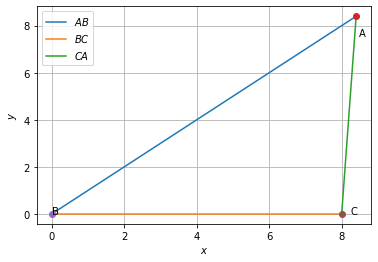
\includegraphics[width=\columnwidth]{solutions/7/Fig1.png}
%     \caption{$\triangle ABC$}
%     \label{constr/7/fig:$\triangle LMN$}
% \end{figure}

 
 
 